\documentclass[12pt,a4paper]{article}
% Set paper dimension
\usepackage[
  top=2cm,
  bottom=2cm,
  left=2cm,
  right=2cm,
  headheight=17pt, % as per the warning by fancyhdr
  includehead,includefoot,
  heightrounded, % to avoid spurious underfull messages
]{geometry}
\usepackage[english]{babel}
\usepackage[utf8]{inputenc}
\usepackage{graphicx}
\graphicspath{ {images/} }
\usepackage{amsmath}
\usepackage{mathtools}
\usepackage{amsfonts}
\usepackage{amssymb}
\usepackage{fancyhdr}
\usepackage{wrapfig}
\usepackage{lscape}
\usepackage{rotating}
\usepackage{epstopdf}
\usepackage{glossaries} 
\usepackage{float}
\usepackage{paralist}

% For the revision table
\usepackage[table]{xcolor}
\setlength{\arrayrulewidth}{0.5mm}
\setlength{\tabcolsep}{12pt}
\renewcommand{\arraystretch}{1.5}
\renewenvironment{enumerate}[1]{\begin{compactenum}#1}{\end{compactenum}}

\usepackage{hyperref}
 % Margins
\topmargin=-0.1in

% Headings
\pagestyle{fancy}
\fancyhf{}
\rhead{\textbf{Page} \thepage}
\lhead{Software Requirements Specification for Lunar Rover Mapping Robot}

\pagenumbering{roman}

\begin{document}
	\begin{titlepage}
		\centerline{\rule{6.5in}{4pt}}
		\vspace*{0.5in}
		\begin{center}
			{\fontfamily{cmr}\selectfont
				{\fontsize{33}{40}\selectfont \textbf{Software Requirements Specification}}\\
				\vspace*{0.5in}
				{\fontsize{20}{40}\selectfont for}\\
				\vspace*{0.5in}
				{\fontsize{33}{40}\selectfont \textbf{Lunar Rover Mapping Robot}}\\
				\vspace*{0.65in}
				{\fontsize{18}{40}\selectfont Version 2.0}\\
				\vspace*{2.5cm}
				{\fontsize{25}{40}\selectfont \textbf{Group: UG12}}\\
				\vspace*{2.5cm}
                \begin{figure}[H]
                \centering
                
\includegraphics[width=0.5\textwidth]{UofA.jpg}
              \end{figure}
              \vspace*{\fill}
			}
		\end{center}
		\centerline{\rule{6.5in}{4pt}}
	\end{titlepage}
	
	\newpage
	
	\tableofcontents
	
    \newpage
   	
	\noindent{\fontsize{16}{40}\textbf{Revision History}}
	\begin{center}
	\begin{tabular}{ |p{2cm}|p{3cm}|p{9cm}|  }
	\hline
	\rowcolor{lightgray}
	Version & Date &Reason for changes \\
	\hline
	1.0 & 22/8/2017 &Initial draft \\
    \hline
	2.0 & 28/10/2017 &Final version \\
	\hline
	\end{tabular}
	\end{center}
    
    \vspace{50px}
    \listoffigures
	
	\newpage
	
    	\pagenumbering{arabic}
	
	\section{Introduction}
	\subsection{Purpose}
This document details the software requirements for the Lunar Rover Mapping Robot Project. It presents the detailed description of the purpose for the system and will explain system features, external interfaces, and non-functional requirements. This document is a guide for developing the initial version of the project and will be proposed to the customer for its approval.

	\subsection{Intended Audience}
   	This document is intended to be read by both the project client and the project developers. For the client, it specifies what the client should expect of the finished product. For developers, it specifies what features need to be completed in order for the project to be considered complete.

	\subsection{Project Scope}
	There are two main objectives of the product specified in this document. The primary objective of the product is to demonstrate a solution, that is within the available budget and capabilities of the organization, in accomplishing the remaining two challenges outlined in the \textbf{Google Lunar XPRIZE}\hyperlink{googlelunarxprize} {[1]}, (\textbf{1}) robot must travel 500 meters on the surface of the Moon and (\textbf{2}) transmit high-definition video and images back to earth, accomplishing this objective will give the organization the edge in winning the prize money of US\$20 million. The secondary objective is to survey a particular area and locate the specific location of the remnants of the Apollo 17 landing site from December 1972 \hyperlink{apollo17} {[2]} and provide precise measurements of the tracks that lead to/from it, accomplishing this objective will satisfy the organization's interest.
    
	\newpage
	\section{Overall Description}
	\subsection{Product Perspective}
    This SRS document presents the proposed software requirements for a Lunar Rover Mapping Robot prototype. The product consists of two major components, the controller and the mapping robot. These components interact with each other as shown in figure \ref{fig:sys1}. The controller, which is operated remotely by a human operator through use of a GUI, sends commands to the robot for it to execute. The mapping robot will send sensor data from the Moon to the controller to be processed.
    \begin{figure}[h]
        \centering
        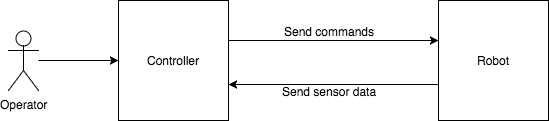
\includegraphics[scale=0.7]{SRS_product_perspective}
        \caption{Operator and subsystem interaction}
        \label{fig:sys1}
    \end{figure}   
	\subsection{Product Features}
     Major features of the Lunar Rover Mapping Robot specify that 
   \begin{itemize}
\item The system will display the entire survey area in real-time, including with the current location of the vehicle, the mapped and unmapped regions, debris and radiation area;
\item The system will store and read the mapping data in \textbf{Extensible Markup Language} (\textbf{XML}) format;
\item The system will enable the operator to zoom in and out on a particular area on the map;
\item The system will enable the operator to move the robot to a specific point on the map;
\item The system will enable the operator to mark \textbf{No-Go-Zones} (\textbf{NGZ}) on the map;
\item The system will provide manual or autonomous control of the mapping robot to the operator;
\item The system will enable the operator to stop the vehicle immediately;
\item The system will be capable of detecting objects to avoid collision or minimize the collision force.
\end{itemize}

\subsection{User Classes and Characteristics}
    
Those interacting with the system will be knowledgeable about the system, how it operates, and it's capabilities. They will be familiar with the functionality of the system, such as sensors and actuators, and how they interact with one another. These users will have unrestricted control over the robot. They will control the robot remotely from Earth.
    
	\subsection{Operating Environment}
Operators will run the controller application on their own computers and connect to the robot wirelessly.
As the controller works on any platform with the Java running environment, the operator’s computer is required to have Java installed.
        
\subsection{Design and Implementation Constraints}
    
The system will be coded as an event-driven program.  A Handler module will be used for handling event command and sensor data transfers between the controller and the robot. The low-level functionality will be managed by a separate Robot module. Queues are used to communicate messages between modules. As an emergency stop button is needed, the priority of received messages must be considered.\\
The LeJOS operating system for the Lego Mindstorms EV3 will be used to interact with the robot.

	\subsection{User Documentation}
    
    	Demonstration will be provided to operators by developers as a tutorial for the correct usage of the system.  The demonstration will include how the controller connect to the robot side, and how to control the robot manually or autonomously through the controllers. 
        
	\subsection{Assumption and Dependencies}
    
    We assume that there will be minimal communication delay between the computer/controller and the robot, which will be on the surface of the Moon. We also assume that objects found on the \textbf{A1} paper map will be 3D objects with sizes that are capable of being accurately detected by the sensors. In addition, we assume that the organization would provide us with a \textbf{document type definition} (\textbf{DTD}) for the mapping data and that there are no restrictions on how many wheels the robot should have.
    
	\newpage
    
	\section{User Requirements}
    \subsection{UR 01: Survey Map}
    \textbf{Description}: The system map shall be able to show found features, current location of the vehicle, and distinguish between mapped and unmapped regions, all in real time.\\
    \textbf{Rationale}: It is vital to the system to be able to see the map and interact with the robot.\\
    \textbf{Acceptance Criteria}: Real time: Without significant delay. Map details, including features, vehicle location and mapped/unmapped areas, shall be clearly visible. \\
    \textbf{Priority}: High.\\
    \textbf{Source}: Client Project Specification\\
    
    \subsection{UR 02: Map Manipulation}
    \textbf{Description}: The map needs to be able to be imported and exported. \\
    \textbf{Rationale}: Exporting means that the map data acquired by the robot can be processed and used externally. Importing means that the robot can take advantage of previous work.\\
    \textbf{Acceptance Criteria}: The map export must conform to the DTD. The map import must be able to import any XML file conforming to the DTD and successfully show it on screen.\\
    \textbf{Priority}: Medium.\\
    \textbf{Source}: Client Project Specification.\\
    
    \subsection{UR 03: Operating the Robot}
    \textbf{Description}: The operator must be able to instantly stop the robot. The operator shall be able to designate a location for the vehicle to immediately move to.\\
    \textbf{Rationale}: The operator needs to be able to stop the robot instantly for the safety of the robot. The operator needs to control where the robot goes.\\
    \textbf{Acceptance Criteria}: "Stop" means no robot motion. "Immediately" means as soon as communication allows. It shall be able to stop at any time.\\
    \textbf{Priority}: High\\
    \textbf{Source}: Client Project Specification.\\
    
    \subsection{UR 04: Safety}
    \textbf{Description}: The robot must not collide with anything with any significant force.\\
    \textbf{Rationale}: This may damage the robot and surroundings.\\
    \textbf{Acceptance Criteria}: The object being collided with shall not move more than 2 cm.\\
    \textbf{Priority}: Medium\\
    \textbf{Source}: Client Project Specification.\\
    
    \newpage
    \section{System Features}
    \subsection{SF 01: Manual Control}
    \textbf{Description}: The system shall enable manual control mode. In manual mode, the user has control over the robots movement through the UI. Both modes includes being able to stop the vehicle at any time.\\
    \textbf{Rationale}: Manual mode is necessary in case something goes wrong with the autonomous mode, or the users judgment is necessary.\\
    \textbf{Acceptance Criteria}: This requirement can be verified in part by entering manual mode and verifying that the robot is being controlled through user input.\\
    \textbf{Priority}: High\\
    \textbf{Source}: UR 03, UR 04\\
    \textbf{Functional Requirements}: \begin{enumerate}
    \item GUI Design.
    \item Robot movement control.
    \item Communication between robot and program.
    \end{enumerate}
    
  
    \subsection{SF 02: Autonomous Control}
    \textbf{Description}: The system shall enable autonomous control mode. In autonomous mode, the user will set a path and the robot will determine the best path to use and direct itself there. While in autonomous mode, the robot will avoid hard collisions with objects and avoid craters, debris and radiation areas.
    In manual mode, the user has control over the robots movement through the UI. Both modes includes being able to stop the vehicle at any time.\\
    \textbf{Rationale}: Autonomous mode is necessary for the robot to move without the user specifying every step. This is useful because the robot can make decisions quickly and efficiently.\\
    \textbf{Acceptance Criteria}: This requirement can be verified by entering autonomous mode and verifying that the robot can navigate its own way through the terrain.\\
    \textbf{Priority}: Medium.\\
    \textbf{Source}: UR 03.\\
    \textbf{Functional Requirements}: \begin{enumerate}
    \item AI path finding
    \item GUI destination selection.
    \end{enumerate}
    
	\subsection{SF 03: Mapping}
    \textbf{Description}: The system shall provide support for mapping functions. The user can designate No Go Zones (NGZ) and points that the robot should navigate to. The user shall also be able to interact with the map, including zooming. The map shall be in XML format and the system shall both read and write to the map. A partial map needs to be able to be uploaded and used. The robot shall also be able to sense obstacles and features and have them displayed on the map.\\
	\textbf{Rationale}: The user needs to be able to navigate the lunar rover around the Moon in manual mode, as well as set, monitor and correct progress in autonomous mode. The map allows these to happen.\\
    \textbf{Acceptance Criteria} This requirement can be verified by uploading a partial map and updating the map with new information from the robot or the user.\\
    \textbf{Priority}: High.\\
    \textbf{Source}: UR 01, UR 02.\\
    \textbf{Functional Requirements}: 
    \begin{enumerate}
    \item Internal map storage.
    \item XML importing and exporting.
    \item GUI Map display.
    \item Robot sensors
    \end {enumerate}
    
    \newpage
    
	\section{External Interface Requirements}
	\subsection{User Interfaces}
	Users will interface with the software via an Java graphical user interface. The interface is composed by three sections, which are controller section, map display section and switch section. User can manually control the robot to send forward, backward, turn clockwise, turn anticlockwise and emergency stop in controller section. The map will be shown to the user in map section and user can adjust the size of the map by zoom in/out. The map can be exported via "save" button. User can also switch the robot into automatic mode or manual mode. \ref{fig:gui}.

\begin{figure}[h!]
\centering
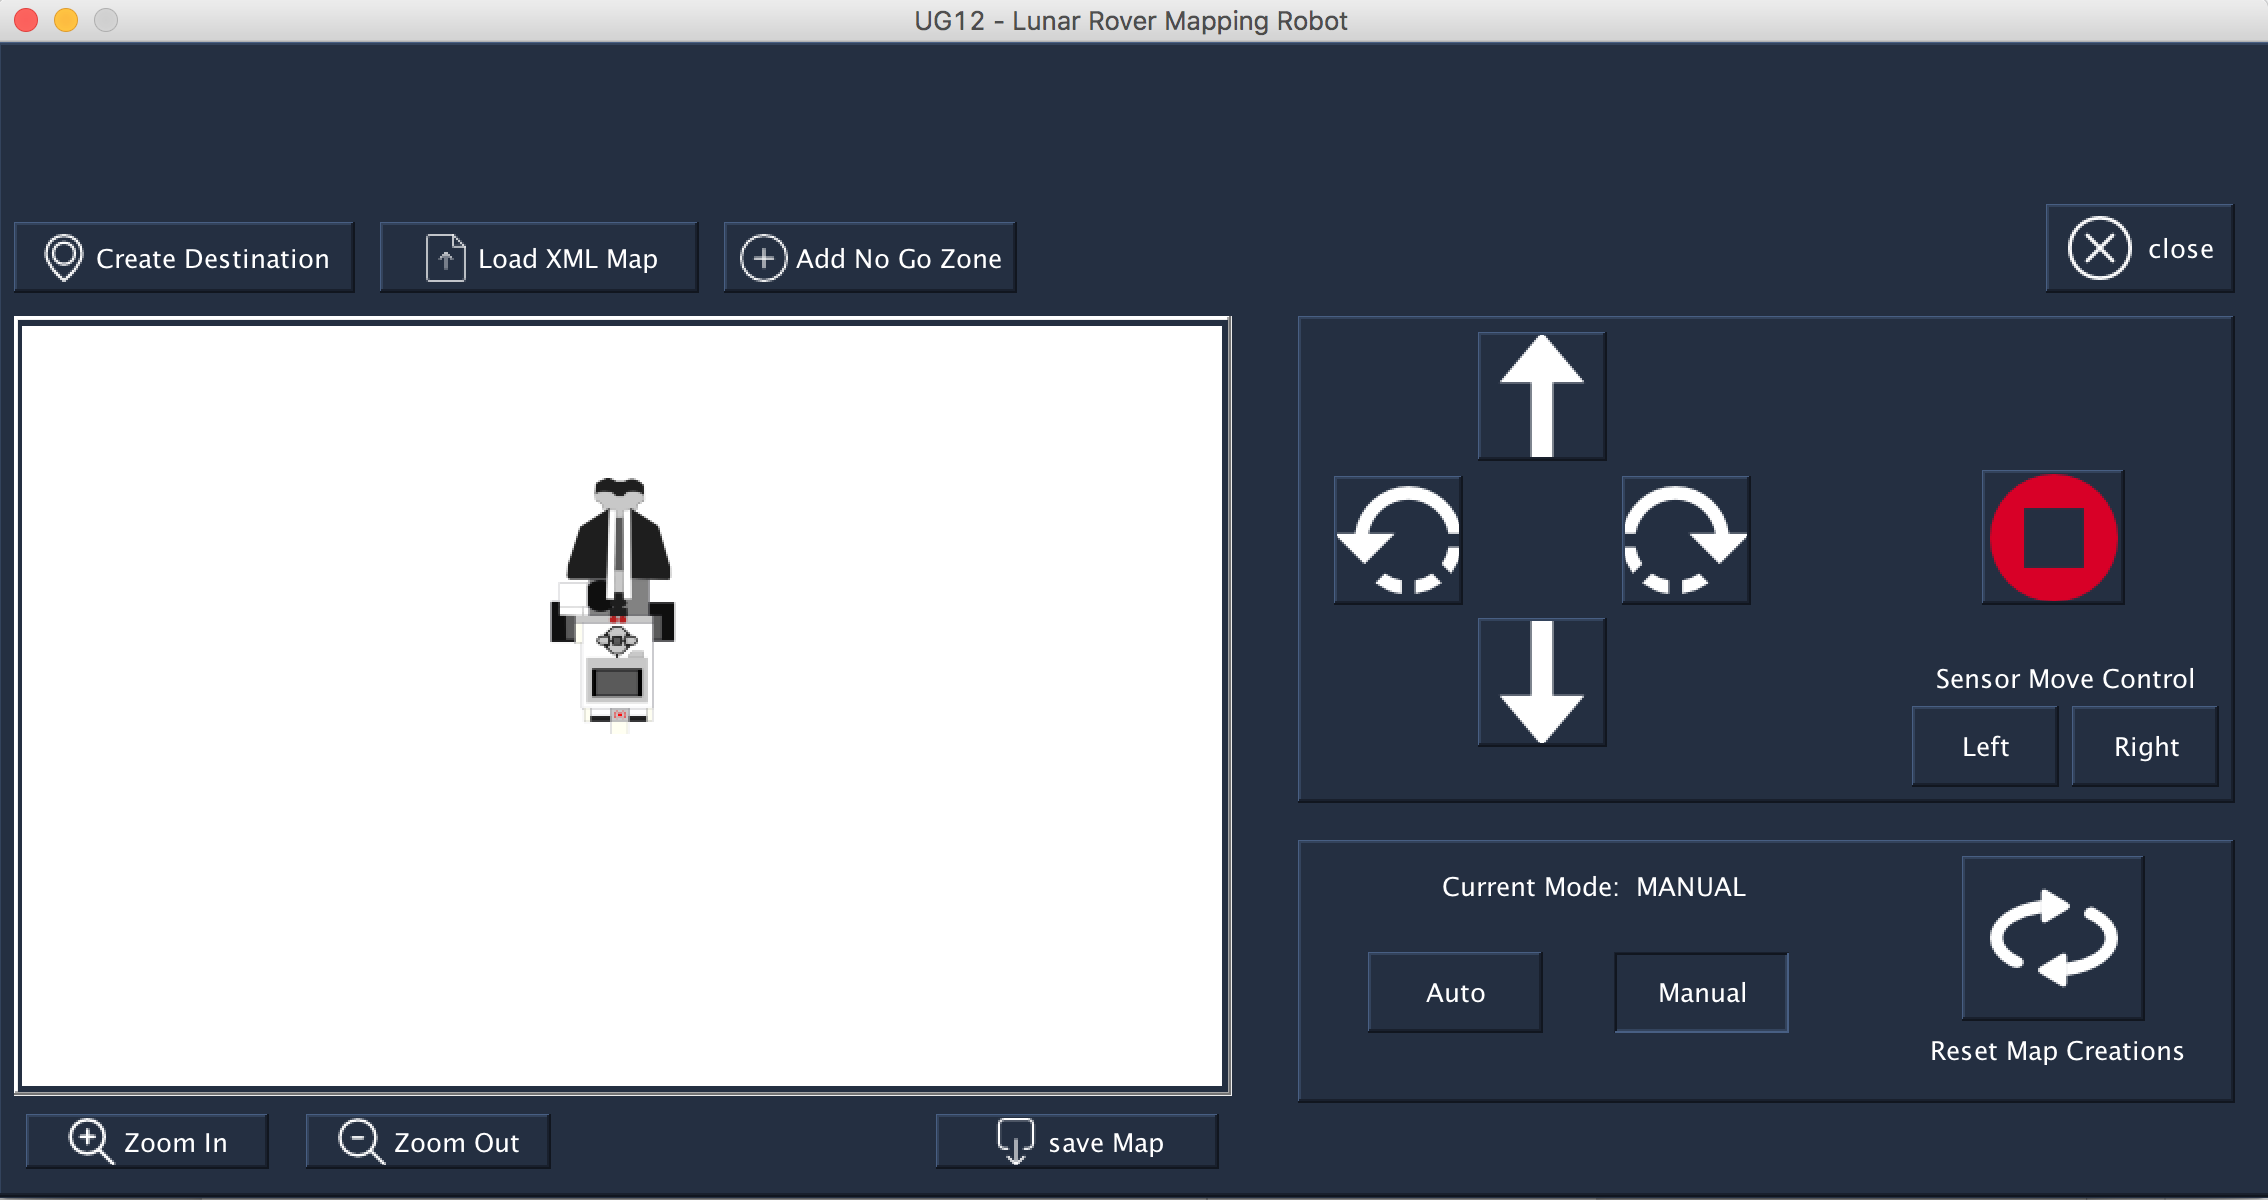
\includegraphics[width=0.7\textwidth]{GUI}
\caption{GUI}
\label{fig:gui}
\end{figure}

	
	\subsection{Hardware Interfaces}
    The robot with which the software interfaces will have two motor-driven wheels to provide control over the motion of the robot. The robot will communicate sensor data back to the software.
	\subsection{Software Interfaces}
    The software will connect to a Lego Mindstorms EV3 unit running the LeJOS operating system. The connection will be made using the Java RMI mechanism supported by LeJOS.
	\subsection{Communications Interfaces}
    The software will communicate with the robot over a wireless network connection. The connection may be maintained over Bluetooth or WiFi standards.
	\newpage
	\section{Other Non-functional Requirements}
	\subsection{Performance Requirements}
    \subsubsection{NF-R01: Survey Speed}
    \textbf{Description} The robot must be able to complete a survey of the demo in less than 20 minutes.\\
    \textbf{Rationale} The final demonstration of the robot will be no longer than 20 minutes, so must be able to complete an autonomous survey with in that time, and ideally in much less.
    \subsubsection{NF-R02: Real-Time Communication} 
    \textbf{Description} The rover must be able to react to commands and send feed back in real time.\\
    \textbf{Rationale} When under manual control, the rover needs to react to updates in commands to provide smooth motion. When under autonomous mode, the rover must respond to any emergency commands. The rover must also relay feedback promptly to aid in pathfinding decisions.
	\subsection{Safety Requirements}
    \subsubsection{NF-R03: Robot Safety}
    \textbf{Description} The Rover must suffer no damage to its equipment, whether from falling into a crater, hitting a physical obstacle, or by any other means. \\
    \textbf{Rationale} The Lunar Rover will be operating on the surface of the moon, controlled remotely from Earth. If damage occurs, there will be no way to repair or recover the Rover. \\

\subsection{Security Requirements}
\textbf{Description} The robot must be appropriately secured.\\
    \textbf{Rationale} As this is a prototype, security protocols will not be implemented.\\

	\subsection{Software Quality Attributes}
    \subsubsection{NF-R04: Modular Design}
    \textbf{Description} The software will be made as separate modules that communicate between each other.\\
    \textbf{Rationale} Using a modular design will allow each module to be modified or replaced without significantly affecting other modules, should changes need to be made to the robot or the mapping system.
	\newpage
	\section*{Appendix A: Glossary}
	\addcontentsline{toc}{section}{Appendix A: Glossary}
    \subsection*{Acronyms}
		\begin{flalign*}
        &\textbf{DTD}	&&\text{Document Type Definition}&&&&&\\
        &\textbf{NGZ}	&&\text{No-Go-Zones}&&&&&\\
        &\textbf{SRS }	&&\text{Software Requirements Specification}&&&&&\\
        &\textbf{UI}		&&\text{User Interface}&&&&&\\
        &\textbf{XML}	&&\text{Extended Markup Language}&&&&&\\
        \end{flalign*}
    \section*{References}
	\addcontentsline{toc}{section}{References}
	\hypertarget{googlelunarxprize}{[1] Google Lunar XPRIZE. 2017. \emph{Google Lunar XPRIZE}. [ONLINE] Available at: \url{https://lunar.xprize.org}. [Accessed 21 August 2017].}\\ \\
	\hypertarget{apollo17}{[2] Wikipedia. 2017. \emph{Apollo 17}. [ONLINE] Available at: \url{https://en.wikipedia.org/wiki/Apollo_17}. [Accessed 21 August 2017].} 
\end{document}